%%%%%%%%%%%%%%%%%%%%%%%%%%%%%%%%%%%%%%%%%%%%%%%%%%%%%%%%%%%%%%%%%%%%%%%%%%%%%%%%%%
\begin{frame}[fragile]\frametitle{}

\begin{center}
{\Large Sequence Tagging}

(Ref: https://www.coursera.org/learn/language-processing/lecture/cNdwa/hidden-markov-models )
\end{center}
\end{frame}


 %%%%%%%%%%%%%%%%%%%%%%%%%%%%%%%%%%%%%%%%%%%%%%%%%%%%%%%%%%%%%%%%%%%%%%%%%%%%%%%%%%
\begin{frame}[fragile]
  \frametitle{Sequence}
  \begin{itemize}
  \item Problem: Given a sequence of tokens, infer the most probable 
sequence of labels for these tokens. 
\item Examples: part of speech tagging, named entity recognition 
  	  \end{itemize}
 \end{frame} 


 %%%%%%%%%%%%%%%%%%%%%%%%%%%%%%%%%%%%%%%%%%%%%%%%%%%%%%%%%%%%%%%%%%%%%%%%%%%%%%%%%%
\begin{frame}[fragile]
  \frametitle{Approaches to sequence labeling}
  \begin{itemize}
  \item Rule-based models (example: EngCG tagger)
  \item Separate label classifiers for each token
  \item Sequence models (HMM, MEMM, CRF)
  \item Neural networks
  	  \end{itemize}
 \end{frame} 
 
 
  %%%%%%%%%%%%%%%%%%%%%%%%%%%%%%%%%%%%%%%%%%%%%%%%%%%%%%%%%%%%%%%%%%%%%%%%%%%%%%%%%%
\begin{frame}[fragile]
  \frametitle{PoS tagging with Hidden Markov Model (HMM)}
  \begin{itemize}
  \item $x = x_1,\ldots,x_T$ is sequence of words (input)
    \item $y = y_1,\ldots,y_T$ is sequence of their corresponsing tags (labels)
    \item We need to find the most probable sequence of tags given 
the sentence:
\item  $y = argmax_y p(y|x) = argmax_yp(x,y)$  
  	  \end{itemize}
 \end{frame} 

  %%%%%%%%%%%%%%%%%%%%%%%%%%%%%%%%%%%%%%%%%%%%%%%%%%%%%%%%%%%%%%%%%%%%%%%%%%%%%%%%%%
\begin{frame}[fragile]
  \frametitle{Hidden Markov Model (HMM)}
  \begin{itemize}
\item Joint probability, apply product rule $p(x,y) = p(x|y)p(y) \approx \Pi p(x_t|y_t)p(y_t|y_{t-1})$  , where x is observable and y is hidden
\item Markov assumption: $p(y) \approx \Pi p(y_t | y_{t-1} )$ Probabilty of next given the previous.
\item Output independence: $p(x|y) \approx \Pi p(x_t | y_{t} )$ probability of input given the output.
  	  \end{itemize}
 \end{frame} 
 
 
%%%%%%%%%%%%%%%%%%%%%%%%%%%%%%%%%%%%%%%%%%%%%%%%%%%%%%%%%%%%%%%%%%%%%%%%%%%%%%%%%%
\begin{frame}[fragile]
  \frametitle{Text generation in HMM}
  Assume that the text is generated in the following manner: 
  \begin{itemize}
\item One chooses the next PoS tag given the previous tag.
\item Given the current tag, one generates another word
\item Thus, the neighboring words do not depend on each other, but 
they depend on the underlying tags. 
  	  \end{itemize}
 \end{frame}

 
    %%%%%%%%%%%%%%%%%%%%%%%%%%%%%%%%%%%%%%%%%%%%%%%%%%%%%%%%%%%%%%%%%%%%%%%%%%%%%%%%%%
\begin{frame}[fragile]
  \frametitle{Text generation in HMM: an example}
Phase I:
\begin{center}
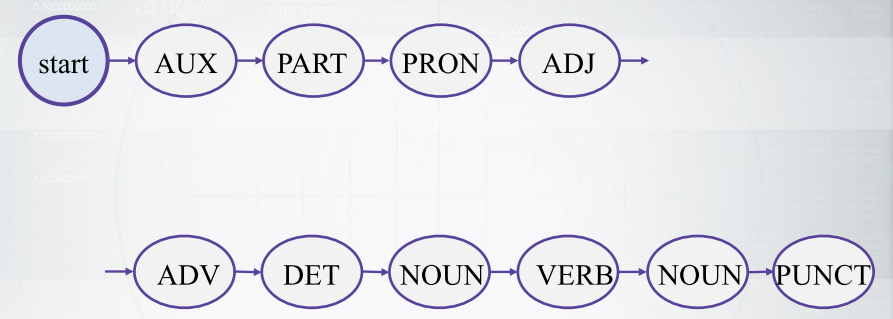
\includegraphics[width=0.8\linewidth,keepaspectratio]{tag1}
\end{center}
 \end{frame} 
  
%%%%%%%%%%%%%%%%%%%%%%%%%%%%%%%%%%%%%%%%%%%%%%%%%%%%%%%%%%%%%%%%%%%%%%%%%%%%%%%%%%
\begin{frame}[fragile]
  \frametitle{Text generation in HMM: an example}
Phase II:
\begin{center}
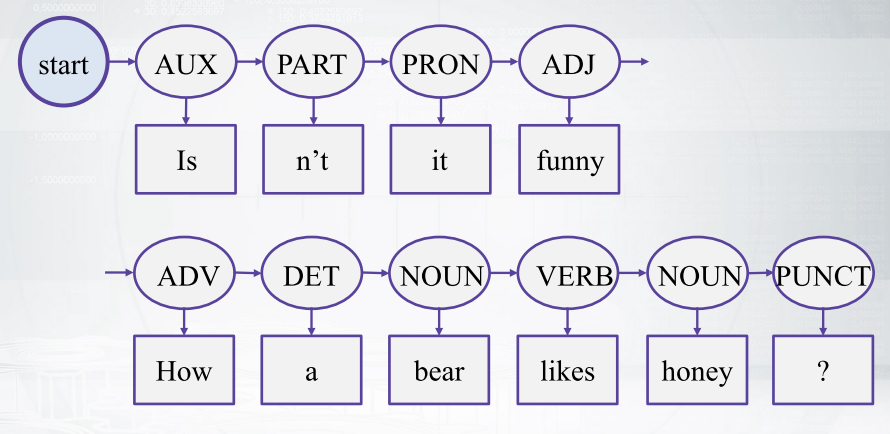
\includegraphics[width=0.8\linewidth,keepaspectratio]{tag2}
\end{center}
 \end{frame} 
  
 %%%%%%%%%%%%%%%%%%%%%%%%%%%%%%%%%%%%%%%%%%%%%%%%%%%%%%%%%%%%%%%%%%%%%%%%%%%%%%%%%%
\begin{frame}[fragile]
  \frametitle{Viterbi algorithm: what are the most probable tags?}
Language can be ambousus as tags for womse workds can be confusing. The same output sentence can be generated by different
sequences of hidden states:
\begin{center}
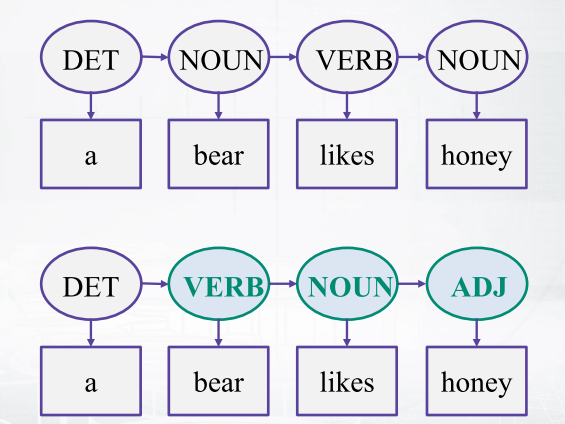
\includegraphics[width=0.6\linewidth,keepaspectratio]{tag3}
\end{center}
 \end{frame} 
  
  
%%%%%%%%%%%%%%%%%%%%%%%%%%%%%%%%%%%%%%%%%%%%%%%%%%%%%%%%%%%%%%%%%%%%%%%%%%%%%%%%%%
\begin{frame}[fragile]
  \frametitle{Decoding in HMM}
Phase II:
\begin{center}
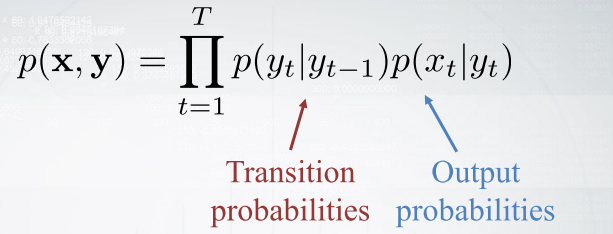
\includegraphics[width=0.8\linewidth,keepaspectratio]{tag4}
\end{center}

What is the most probable sequence of hidden states? 

$p(x,y) = p(x|y)p(y) \approx \Pi p(x_t|y_t)p(y_t|y_{t-1})$

Solve this problem efficiently using dynamic programming!
 \end{frame} 
  
  
  %%%%%%%%%%%%%%%%%%%%%%%%%%%%%%%%%%%%%%%%%%%%%%%%%%%%%%%%%%%%%%%%%%%%%%%%%%%%%%%%%%
\begin{frame}[fragile]
  \frametitle{Summary: HMM}

\begin{center}
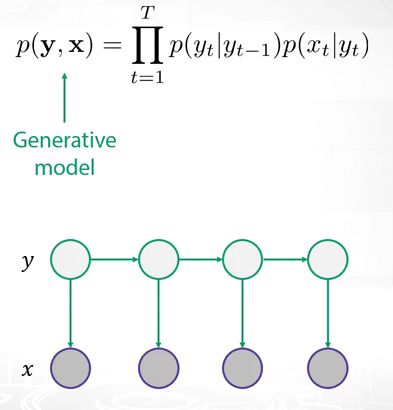
\includegraphics[width=0.5\linewidth,keepaspectratio]{tag5}
\end{center}

  \begin{itemize}
\item Every arrow is about some particular probability in the formula. 
\item So we have transition probabilities going from one y to the next one, and we have output probabilities that go to x variables
  	  \end{itemize}
 \end{frame} 
 
   
  %%%%%%%%%%%%%%%%%%%%%%%%%%%%%%%%%%%%%%%%%%%%%%%%%%%%%%%%%%%%%%%%%%%%%%%%%%%%%%%%%%
\begin{frame}[fragile]
  \frametitle{Maximum entropy Markov Models MEMM}

\begin{center}
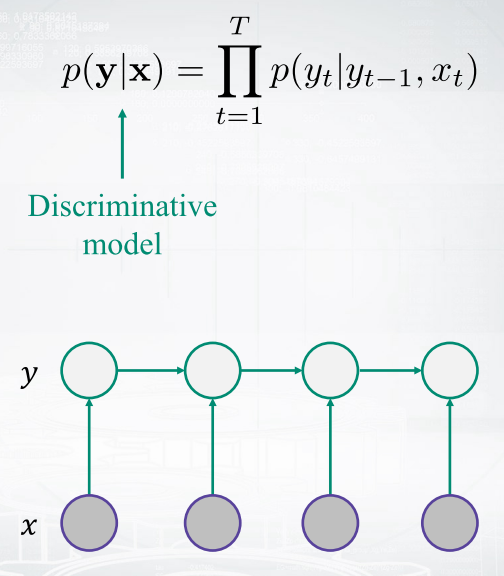
\includegraphics[width=0.5\linewidth,keepaspectratio]{tag6}
\end{center}

  \begin{itemize}
\item Similar to HMM
\item Its  Discriminative. It models the conditional probability of y given x
\item  Only one thing has changed. You have now the arrows going from x to ys.
  	  \end{itemize}
 \end{frame} 
 
   %%%%%%%%%%%%%%%%%%%%%%%%%%%%%%%%%%%%%%%%%%%%%%%%%%%%%%%%%%%%%%%%%%%%%%%%%%%%%%%%%%
\begin{frame}[fragile]
  \frametitle{Maximum entropy Markov Models MEMM}

\begin{center}
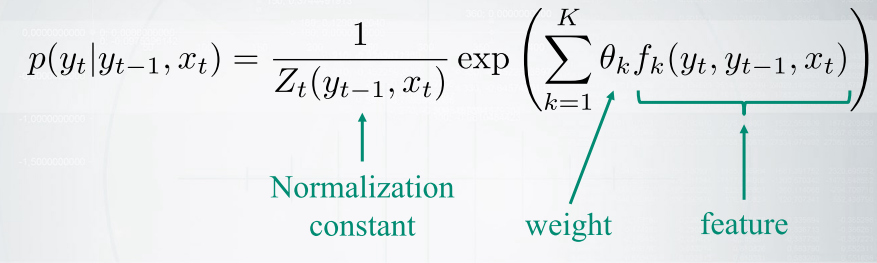
\includegraphics[width=0.8\linewidth,keepaspectratio]{tag7}
\end{center}

  \begin{itemize}
\item The vectorization is a little bit different. We have the probabilities of current tag given the previous tag, and the current x. 
\item  It says that the text is observable and we just need to produce the probabilities for our hidden variables, y.
  	  \end{itemize}
 \end{frame} 
  
    %%%%%%%%%%%%%%%%%%%%%%%%%%%%%%%%%%%%%%%%%%%%%%%%%%%%%%%%%%%%%%%%%%%%%%%%%%%%%%%%%%
\begin{frame}[fragile]
  \frametitle{Conditional Random Field (linear chain)}

\begin{center}
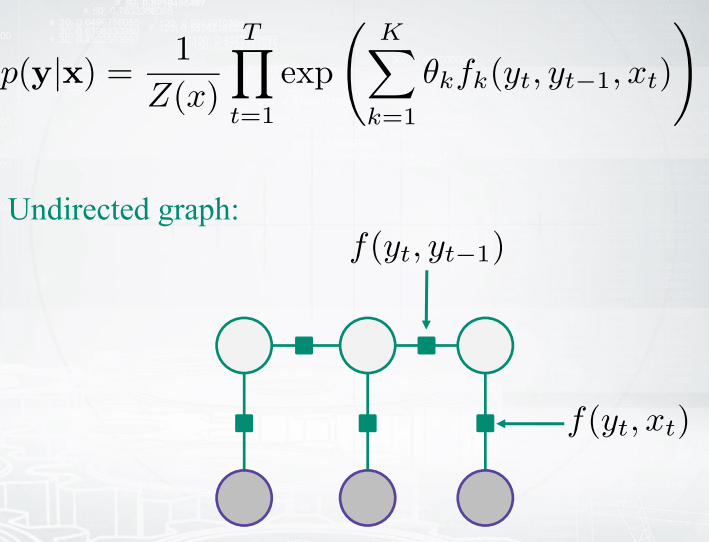
\includegraphics[width=0.6\linewidth,keepaspectratio]{tag8}
\end{center}

 \end{frame} 
 
     %%%%%%%%%%%%%%%%%%%%%%%%%%%%%%%%%%%%%%%%%%%%%%%%%%%%%%%%%%%%%%%%%%%%%%%%%%%%%%%%%%
\begin{frame}[fragile]
  \frametitle{Conditional Random Field (general form)}

\begin{center}
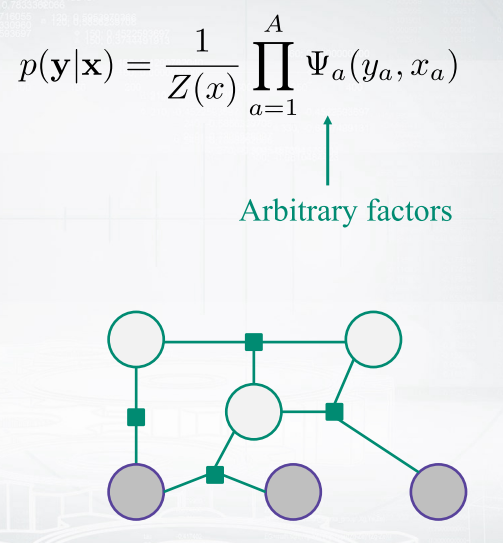
\includegraphics[width=0.6\linewidth,keepaspectratio]{tag9}
\end{center}

 \end{frame} 
  
  
  